\documentclass[10pt,twocolumn,letterpaper]{article}

\usepackage{iccv}
\usepackage{times}
\usepackage{epsfig}
\usepackage{graphicx}
\usepackage{amsmath}
\usepackage{amssymb}

% Include other packages here, before hyperref.

% If you comment hyperref and then uncomment it, you should delete
% egpaper.aux before re-running latex.  (Or just hit 'q' on the first latex
% run, let it finish, and you should be clear).
\usepackage[pagebackref=true,breaklinks=true,letterpaper=true,colorlinks,bookmarks=false]{hyperref}


\iccvfinalcopy % *** Uncomment this line for the final submission
\def\iccvPaperID{****} % *** Enter the ICCV Paper ID here
\def\httilde{\mbox{\tt\raisebox{-.5ex}{\symbol{126}}}}

% Pages are numbered in submission mode, and unnumbered in camera-ready
\ificcvfinal\pagestyle{empty}\fi
\begin{document}

%%%%%%%%% TITLE
\title{Project Proposal: Job Recommender System}

\author{Jimmy Lin\\
Univeristy of Texas At Austin\\
Austin, the United States\\
{\tt\small \url{JimmyLin@utexas.edu}}
% For a paper whose authors are all at the same institution,
% omit the following lines up until the closing ``}''.
% Additional authors and addresses can be added with ``\and'',
% just like the second author.
% To save space, use either the email address or home page, not both
%\and
%Pradeep Ravikumar\\
%University of Texas At Austin\\
%Austin, the United States\\
%{\small\url{pradeep.ravikumar@gmail.com}}
}

\maketitle
% \thispagestyle{empty}

%%%%%%%%% ABSTRACT
\begin{abstract}
    As the labor market expands increasingly, the investigation for
    automatically matching job to person meets its high in recent years.
    A formal job recommendation system is expected to provide recommendation
    to employers by which applicant deserves being noticed and employees by
    which company suits itself most. For startup, the most economic
    combination of predictors is blended to generate the ultimate output. In this
    project, we investigate the methods used in job recommendation system and
    implement a micro job recommendation system. 
\end{abstract}

%%%%%%%%% BODY TEXT
\section{Introduction}

As the labor market expands increasingly, the investigation for automatically
matching job to person meets its high in recent years. Formally, job
recommendation refers to bi-directional service. That is, it is supposed to
provide suitable job applicants to companies or job hunters and in the
meanwhile, offer suitable job position to job applicants. 

To effectively automate the job recommendation, a system is supposed to
efficiently extract quantitative information from large number of curriculum
vitaes and job requirements. This may involve in some natural language
processing techniques. And after that, that system must precisely evaluate
the suitability between job and user, based on which correct recommendation is
generated. 

In this project, we investigate the methods used in recommendation system and
implement a micro job recommendation system. The rest of this report is
organized as follows: section 2 discuss the related works; section 3 presents
the description of dataset; section 4 introduces the methods to be used for
project startup, but not in details.  

\section {Related Works}
Job Recommender System (JRS) is rather similiar to the Movie
Recommender System (MRS), in the sense that JRS matches job to user according
to the description of job and user, while MRS associates movie to user based on
the profiles of movie and user. Such semantical analogy provides heuristics
 of applying existing methods that have already earned huge achievements in
 MRS on the JRS. To circumvent cold start-up, at least in the initial stage,
 we restrict our attention only on the methods or combination of methods, from
 Netflix Prize Challenge, with great economy in practice. 

The works topped in the Netflix Prize employ the highly similar framework to
achieve movie recommender system. As a part of the final winner, Martin P.
and Martin C. presents such framework in their project report
\cite{Piotte09thepragmatic}. They all estimate the rating $r_{ui}$ of
human over movies. And they all have a general baseline model containing basic
component to be evaluated in all prediators. Based on the baseline, various
predictors incorporate the particular items it exclusively values over the
rating. Hence, each predictor is being fitted in terms of its own
"understanding" of the relationship between user and movie. After fitting all
valuable result, the ultimate prediction of the whole system comes from
summarizing the consequence of all used predictors by certain blending
algorithm.

On the other hand, some of existing job recommender systems exploit original
framework to provide job recommendation service. One well-known framework is
Hybrid Recommendation \cite{LuHG13}. In a pipelined hybrid
recommendation, the result of content-based similarity is fed into a
relation-based algorithm as an additional relation after normalization.

\section {Dataset}
The dataset utilized in this project comes from a Job Recommendation Challenge
posted on \url{kaggle.com}. The provider of this dataset is
\url{CareerBuilder.com}, one of the biggest job recommendation service
providers. This bunch of records, sized of several Gigabytes, include
characterization of users, description of jobs and hundreds of thousands of
job application records.

In outline, the data on users, job postings, and job applications that
users have made to job postings is provided. In total, the applications span
13 weeks. All the job applications are split into 7 groups, each group
representing a 13-day window. Each 13-day window is split into two parts: The
first 9 days are the training period, and the last 4 days are the test period.
The graphical representation demonstrating such splits is illustrated below.

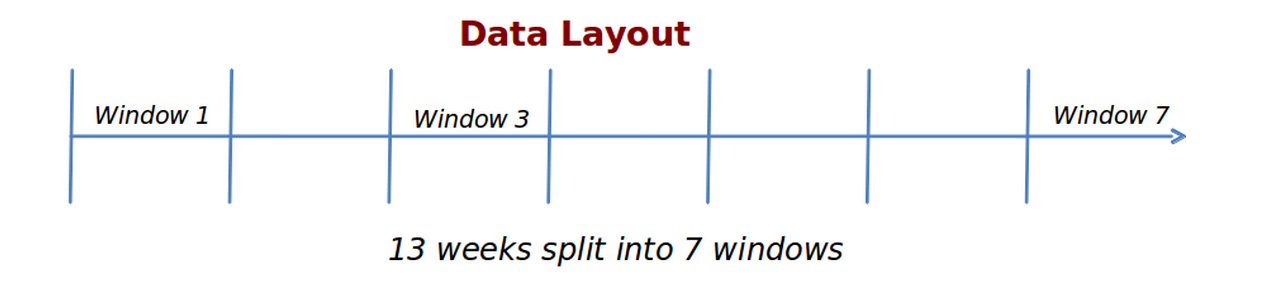
\includegraphics[width=3.3in,height=1.2in]{./dataset/datalayout.png}

Each user and each job posting is randomly assigned to exactly one window.

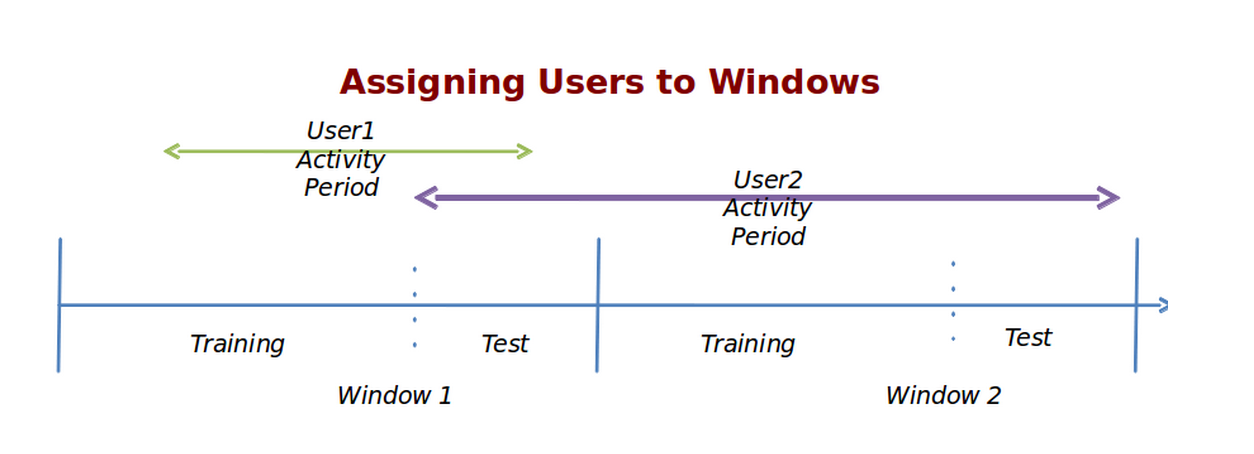
\includegraphics[width=3.3in,height=1.5in]{./dataset/assignusertowindows.png}

Each job is assigned to a window with probability proportional to the time it
was live on the site in that window. Each user is assigned to a window with
probabilty proportional to the number of applications they made to jobs in
that window. In the above image, User1 only made submissions to jobs in
Window 1, and so was assigned to Window 1 with probability 100\%. User2,
however, made submissions to jobs in both Window 1 and Window 2, and so may
have been assigned to either Window1 or Window2.

In each window, all the job applications that users in that window made to
jobs in that window during the 9-day training period. 

In each window, users have been split into two groups, Test group and Train
group. The Test users are those who made 5 or more applications in the 4-day
test period, and the Train users are those who did not.

For each window, the task of prediction is which jobs in that window the Test
users applied for during the window's test period. Note that users may have
applied to jobs from other windows as well, but the only thing needed to be
predicted is which jobs they applied to in their own windows.

\section{Approaches}
In this section, we are going to present the approaches to be used for
matching jobs and persons. The first subsection introduces the methods to
extract machine-understandable features from the raw dataset. And the
whole framework for application prediction, the core of job recommendation, is
indicated in the second part.

\subsection{Data Preprocessing}
The common sense tells us that word description of both person profiles and
job postings are significantly informative in reflecting certain properties of
the job positions and job applicants. For example, the professions employer
expect to job applicants to have and the specialism one job applicant
possess. Therefore, one natural language processing technique is indispensable
to capture the information resident in the textual data. 

We model the preprocessing for textual data as a multi-class categorization
problem. Given a paragraph of job applicant profile, the information, like 
personality, skills possessed, experiences, is supposed to be figured out. And
the treatment to job posting requirements is similar. To resolve this
categorization problem, keyword abstraction technique in the area of natural
language processing can be helpful. Specifically, the TF-IDF algorithm would
work well to categorize the provided textual data for both requirements of job
postings and CVs of job applicants.

\subsection{Baseline Estimation} 
Some models require a simple approximation of the ratings as an element of the
model. We develop one baseline in the following and provide it for the
approximation of the ratings afterwards. 

\begin{equation}
    baseline(u, j) = \mu + b_{baseline,j} (j) + b_{baseline, u} (u)
\end{equation}
where: \\
\hspace*{0.5cm} $\bullet$ $u$ represents the user; \\
\hspace*{0.5cm} $\bullet$ $j$ represents job; \\
\hspace*{0.5cm} $\bullet$ $baseline$ represents for the approximation of
ratings; \\
\hspace*{0.5cm} $\bullet$ $\mu$ is the global rating mean; \\
\hspace*{0.5cm} $\bullet$ $b_{baseline,j}$ for job bias; \\
\hspace*{0.5cm} $\bullet$ $b_{baseline,u}$ for user bias.

Nevertheless, the temporal variables are not taken into consideration in above
baseline. Since proper incorporation of time variable would significantly
enhance the performance \cite{Piotte09thepragmatic}, a time-sensitive baseline
is supposed to be utilized. Hence, the baseline predictor for user $u$' rating
of $i$ at day $t_{ui}$

\begin{equation}
    baseline(u, j) = \mu + b_{j} (t_{uj}) + b_{u} (t_{uj})
\end{equation}
where the $b_{j} (\cdot)$ and $b_{u}(\cdot)$ are real valued function changing
over the time variable $t$, rather than a simply scalar value. 

\subsection{Predictors}
Here we refer to the publications of top five teams in Netflix Challenges and
pick up the most economic combination of predictors. According to the
suggestions from the BellKor's implementation in 2008 \cite{Bell_thebellkor}, 
a high precision of prediction could be generated by combining four basic
predictors. They are respectively: (i) Simufctr with 60 factors, (ii)
Restricted Boltzman Machine with 100 hidden units, (iii) 50 neighbours
K-Nearest Neighbours on 100-unit RBM, (iv) SVD++ with 200-dimensional factor
vectors.

Note that the combination of those predictors listed above does not provide
the optimal result, even with the best blending algorithm, but close to
the optimal one, which consists of hundreds of predictors. Hence, out of the
implementation simplicity, the selected combination of predictors reasonably suffice.

\subsection {Blending Methods}
The key to achieve precise prediction is to use a mixture of multiple
predictors. Nevertheless, the outcome of different blending algorithm would vary
tremendously. That is, an appropriate blending algorithm would significantly
improve the recommendation accuracy. This is true, especially when a large
number of predictors have been employed and improvement on single
predictor will not affect the final result even in a slight degree.

Basically, the list of well-performed blending algorithms occuring in the
Netflix Challenge includes Set Selection Algorithm, Neural Network blending,
and Gradient Boosted Decision Tree (GBDT). Among them, GBDT has turned out to
be the one resulting in the highest outcome improvement.

GBDT is an additive regression model consisting of an ensemble of trees,
fitted to current residuals in a forward step-wise manner. In the traditional
boosting framework, the weak learners are generally shallow decision trees
consisting of a few leaf nodes. GBDT ensembles are found to work well when
there are hundreds of such decision trees.

In this project, a reasonable strategy is to simply implement linear average of
different predictors at first to produce the blended result for its
implementation simplicity. Once all predictors are confirmed to be technically
correct, we can turn our focus on implementing the advanced blending
algorithm, GBDT.


%-------------------------------------------------------------------------

{\small
\bibliographystyle{ieee}
\bibliography{main}
}


\end{document}
